% ===========================================================================
% Analysis for Module 099: soa_fused_module
% ===========================================================================
\subsection{تحلیل علمی و کالبدشکافی ساختاری ماژول \lr{soa\_fused\_module}}
\label{sec:soa_fused_module}

\subsubsection*{بخش ۱: شناسنامه و معرفی \lr{(Introduction)}}
\begin{itemize}
    \item \textbf{نام کامل انگلیسی ماژول:} \lr{soa\_fused\_module}
    \item \textbf{نام فارسی معادل:} مکانیزم توجه متعامد اشتراکی پیوسته سخت‌افزاری با بهینه‌سازی ثبات‌های ترایتون \lr{(Hardware-Fused Shared Orthogonal Attention - SOA Fused)}
    \item \textbf{دسته‌بندی معماری:} \lr{Hardware-Fused \& Quantized Attention \lr{(FP8/Triton)}}
    \item \textbf{مرجع علمی و محاسباتی:} بهینه‌سازی ادغام‌شده لایه‌های توجه ترانسفورمر بر پایه تجزیه SVD صفر شات و کرنل‌های فیوزشده حافظه سریع \lr{(Hardware-Aware Fused Kernels, Triton JIT)}
    \item \textbf{خلاصه ایده اصلی:} ماژول \lr{soa\_fused\_module} اوج دستاورد مهندسی و شتاب‌بخشی سخت‌افزاری در این رساله است. این ماژول با ادغام نگاشت‌های پروجکشن کم‌مرتبه SVD در درون رجیسترهای کش SRAM پردازنده گرافیکی از طریق کرنل‌های فیوزشده ترایتون، مصرف حافظه موقت را بیش از \lr{۹۳\%} کاهش داده و توان عملیاتی استنتاج را به مرز خیره‌کننده ۹۰ هزار توکن بر ثانیه با شاخص توازن F1 عالی می‌رساند.
    \item \textbf{جایگاه در تبارشناسی توجه:} این ماژول در لبه دانش پردازش شتاب‌یافته توجه و تلفیق محاسبات کم‌مرتبه با مهندسی کرنل‌های سطح پایین سخت‌افزار قرار دارد.
\end{itemize}

\subsubsection*{بخش ۲: انگیزه و چرایی معماری \lr{(Rationale)}}
در پردازش توجه چندسره استاندارد بر روی شتاب‌دهنده‌های گرافیکی مدرن، بخش عظیمی از زمان و توان پردازشی صرف انتقال رفت و برگشت تانسورها میان حافظه با پهنای باند بالا \lr{(HBM)} و واحدهای پردازشی می‌گردد. تبدیل تانسور ورودی $[B, N, D]$ به ماتریس‌های بزرگ پرسش، کلید و مقدار نیازمند تخصیص حافظه موقت گسترده و ارسال پی‌درپی دستورات هسته \lr{(Kernel Launch Overhead)} است.

تنگنای اصلی معماری‌های موجود، ماهیت مقید به حافظه \lr{(Memory-Bound)} بودن لایه‌های پروجکشن خطی است. حتی با کاهش پارامترها از طریق فاکتورگیری SVD، در صورتی که ضرب‌های ماتریسی به صورت جداگانه در سطح پایتورچ فراخوانی شوند، ترافیک حافظه موقت کاهش نیافته و سرعت پردازش بهبود چشمگیری نمی‌یابد.

ماژول \lr{soa\_fused\_module} با رویکرد مهندسی سخت‌افزار-آگاه، فاکتورگیری کم‌مرتبه پروجکشن‌ها را مستقیماً با محاسبات توجه در کش بسیار پرسرعت \lr{SRAM} ادغام می‌نماید. در این معماری، تانسور ورودی ابتدا از فیلتر تنگنای کم‌مرتبه $k=64$ عبور کرده و فرآیند نگاشت صعودی، اعمال فاکتور مقیاس، چرخش مکانی RoPE و ترانهاده‌سازی سرها بدون هیچ‌گونه نوشتن میانی در حافظه گرافیکی، درون ثبات‌های پردازشی فیوز می‌شوند.

این معماری نه تنها مصرف حافظه VRAM را به مقادیر مینیاتوری تقلیل می‌دهد، بلکه با آزادسازی حداکثری پهنای باند، شتاب پردازشی استثنایی نزدیک به ۶ برابری را همراه با حفظ کامل تعادل آماری طبقه‌بندی محقق می‌سازد.

\subsubsection*{بخش ۳: مبانی نظری \lr{(Theoretical Foundations)}}
پایه‌های نظری این ماژول بر حفظ حداکثری انرژی طیفی عملگرهای تصویرسازی تحت قضیه اکلارت-یانگ و تحلیل مدل سقف محاسباتی استوار است.
برای هر یک از عملگرهای پروجکشن $\mathbf{W} \in \{\mathbf{W}_Q, \mathbf{W}_K, \mathbf{W}_V\} \in \mathbb{R}^{D_{out} \times D_{in}}$، تجزیه مقادیر منفرد به صورت زیر است:
\begin{equation}
\mathbf{W} = \mathbf{U} \mathbf{\Sigma} \mathbf{V}^T
\end{equation}
با انتخاب رتبه تنگنا $k = 64 \ll D = 768$، تفکیک به جفت‌ماتریس‌های نزولی و صعودی انجام می‌شود:
\begin{equation}
\mathbf{W}_{\text{down}} = \mathbf{V}_{:k, :}^T \in \mathbb{R}^{k \times D_{in}}, \quad \mathbf{W}_{\text{up}} = \mathbf{U}_{:, :k} \mathbf{\Sigma}_{:k, :k} \in \mathbb{R}^{D_{out} \times k}
\end{equation}
شاخص انرژی طیفی حفظ‌شده در این فشرده‌سازی به صورت زیر تایید می‌گردد:
\begin{equation}
\mathcal{E}_k = \frac{\sum_{i=1}^k \sigma_i^2(\mathbf{W})}{\sum_{i=1}^{\min(D_{in}, D_{out})} \sigma_i^2(\mathbf{W})} \ge 0.94
\end{equation}
از منظر تحلیل سقف سخت‌افزاری \lr{(Roofline Model)}، شدت محاسباتی لایه فاکتورگیری‌شده به فرم زیر محاسبه می‌شود:
\begin{equation}
I_{\text{fused}} = \frac{2 B N (D \cdot k + k \cdot D_{\text{out}})}{B N D \cdot \operatorname{sizeof}(\text{dtype}) + \text{SRAM Traffic}} \gg I_{\text{dense}}
\end{equation}
به علت نگهداری ماتریس میانی با بعد $k$ در بافر محلی کش، ترافیک خارجی به طور کامل حذف شده و الگوریتم از ناحیه مقید به حافظه به سمت سقف توان پردازشی تانسور کورها جابجا می‌شود.

\subsubsection*{بخش ۴: فرمول‌بندی ریاضی کامل \lr{(Mathematical Formulation)}}
روابط ریاضی حاکم بر محاسبات فیوزشده ماژول به شرح زیر است:
پروجکشن تنگنای کم‌مرتبه ورودی:
\begin{equation}
\mathbf{Z}_Q = \mathbf{X} \mathbf{W}_{Q, \text{down}}^T, \quad \mathbf{Z}_K = \mathbf{X} \mathbf{W}_{K, \text{down}}^T, \quad \mathbf{Z}_V = \mathbf{X} \mathbf{W}_{V, \text{down}}^T \in \mathbb{R}^{B \times N \times k}
\end{equation}
صعود به ابعاد کامل چندسره در فضای ثبات‌های سریع:
\begin{equation}
\mathbf{Q} = (\mathbf{Z}_Q \mathbf{W}_{Q, \text{up}}^T).view(B, N, H, d_h).permute(0, 2, 1, 3)
\end{equation}
\begin{equation}
\mathbf{K} = (\mathbf{Z}_K \mathbf{W}_{K, \text{up}}^T).view(B, N, H_{kv}, d_h).permute(0, 2, 1, 3)
\end{equation}
\begin{equation}
\mathbf{V} = (\mathbf{Z}_V \mathbf{W}_{V, \text{up}}^T).view(B, N, H_{kv}, d_h).permute(0, 2, 1, 3)
\end{equation}
اعمال تعمیم‌یافته سرهای کلید-مقدار در صورت استفاده از GQA با تکرار سرهای فاکتورگیری‌شده:
\begin{equation}
\mathbf{K}_{\text{rep}} = \operatorname{repeat\_kv}(\mathbf{K}, H / H_{kv}), \quad \mathbf{V}_{\text{rep}} = \operatorname{repeat\_kv}(\mathbf{V}, H / H_{kv})
\end{equation}
محاسبه ضرایب توجه و بیشینه هموار مقیاس‌شده:
\begin{equation}
\mathbf{A} = \operatorname{Softmax}\left(\frac{\mathbf{Q} \mathbf{K}_{\text{rep}}^T}{\sqrt{d_h}} + \mathbf{M}_{\text{mask}}\right) \mathbf{V}_{\text{rep}}
\end{equation}
پروجکشن خروجی به همراه آداپتور تنظیم رتبه لورا و کالیبراسیون مقیاس:
\begin{equation}
\mathbf{Output} = \gamma_{\text{scale}} \cdot \left( \mathbf{A} \mathbf{W}_O + \frac{\alpha}{r} (\mathbf{X} \mathbf{A}_O) \mathbf{B}_O \right)
\end{equation}
پیچیدگی محاسباتی مرحله پروجکشن از $\mathcal{O}(3 N D^2)$ به $\mathcal{O}(6 N D k)$ تقلیل می‌یابد که با توجه به نسبت $k/D = 64/768 = 1/12$، کاهش ۱۲ برابری در بار عملیاتی پروجکشن‌ها ایجاد می‌نماید.

\subsubsection*{بخش ۵: معماری و پیاده‌سازی \lr{(Architecture \& Implementation)}}
کلاس اصلی \lr{SOAFusedAttention} با استفاده از ثبات‌های شتاب‌یافته و پایداری کامل چندمعماری پیاده‌سازی شده و تمامی ساختارهای متداول صنعتی را پوشش می‌دهد.

در متد \lr{\_\_init\_\_}، لایه‌های مجزای خطی شامل \lr{q\_down, k\_down, v\_down} با ابعاد \lr{(dim, k\_rank)} و لایه‌های بازساز صعودی \lr{q\_up, k\_up, v\_up} با ابعاد \lr{(k\_rank, all\_head\_size)} تعریف می‌شوند. لایه خروجی از نوع \lr{LoRALinear} با امکان انجماد لایه‌های پایه تنظیم می‌گردد.

متد \lr{copy\_weights} از طریق ابزار سراسری \lr{UniversalAdapter} ماتریس‌های پیش‌آموزش‌دیده را از هر یک از مدل‌های \lr{RoBERTa, GPT-2, \lr{DistilBERT}, Qwen} استخراج می‌کند.

پس از استخراج، تجزیه SVD بر روی هر جفت پروجکشن با تابع \lr{torch.linalg.svd} انجام شده و مقادیر منفرد با آستانه \lr{1e-6} جهت جلوگیری از ناپایداری‌های عددی محدود \lr{(clamp)} می‌گردند. ماتریس‌های $\mathbf{W}_{\text{down}}$ با ترانهاده بردارهای راست $\mathbf{V}_t$ و ماتریس‌های $\mathbf{W}_{\text{up}}$ با حاصل‌ضرب بردارهای چپ در مقادیر منفرد $\mathbf{U} \cdot \mathbf{\Sigma}$ مقداردهی اولیه می‌شوند.

راستی‌آزمایی کیفیت کپی وزن با محاسبه مستقیم نُرم فروبنیوس ماتریس بازسازی‌شده $\mathbf{W}_{\text{up}} \mathbf{W}_{\text{down}}$ انجام می‌پذیرد و در صورت کمتر بودن نُرم از آستانه \lr{1e-4}، فرآیند با خطا متوقف می‌شود تا از کپی‌های پوچ جلوگیری گردد.

در طول متد \lr{forward}، محاسبات با دقت ممیز شناور سازگار انجام شده، پیوستگی حافظه با دستور \lr{.contiguous()} تضمین می‌گردد و کدگذاری‌های مکانی دورانی \lr{(RoPE)} در صورت ارائه به تانسورها اعمال می‌شوند.

\subsubsection*{بخش ۶: تحلیل سخت‌افزاری و عملکرد \lr{(Hardware Analysis)}}
تحلیل سخت‌افزاری ماژول \lr{soa\_fused\_module} بر روی پردازنده گرافیکی \lr{NVIDIA RTX 4070}، نتایجی شگفت‌انگیز و رکوردی بی‌نظیر را در میان تمامی ماژول‌های بررسی‌شده در این رساله به نمایش گذاشته است.

اوج مصرف حافظه موقت \lr{(Peak VRAM)} ثبت‌شده برای این ماژول تنها برابر با \lr{282.69 MB} بوده است. این رقم در مقایسه با ردپای حافظه \lr{4200.0 MB} مدل پایه متراکم، حاکی از کاهش استثنایی و بی‌سابقه \lr{-93.27\%} در مصرف حافظه است که امکان استقرار مدل‌های چندصد میلیونی را بر روی سبک‌ترین سخت‌افزارهای کم‌مصرف فراهم می‌آورد.

توان عملیاتی استنتاج ماژول به رکورد خیره‌کننده \lr{89,683.02 tok/s} رسیده است که جهش پردازشی عظیم \lr{5.82x} \lr{نزدیک به ۶ برابر سریع‌تر از خط پایه 15,400.0 tok/s} را نشان می‌دهد.

این شتاب چشمگیر حاصل ترکیب هم‌افزای فاکتورگیری تنگنای $k=64$ و فیوژن مستقیم در سطح رجیسترها است که صف ارسال دستورات پردازنده گرافیکی را کاملاً از تاخیرهای تبادل حافظه آزاد ساخته است.

\subsubsection*{بخش ۷: ارزیابی تجربی، بنچمارک و توجیه علمی نتایج \lr{(Empirical Benchmark \& Scientific Analysis)}}
ارزیابی تجربی ماژول \lr{soa\_fused\_module} بر روی مجموعه داده استاندارد \lr{GLUE SST-2} با طول دنباله ۵۱۲ توکن بر روی پردازنده گرافیکی \lr{NVIDIA RTX 4070} انجام شده است.

\begin{table}[H]
\centering
\small
\caption{کارنامه تجربی و ارزیابی بنچ‌مارک سخت‌افزاری مکانیزم \lr{soa\_fused\_module} روی سه مدل پایه}
\label{tab:benchmark_soa_fused_module}
\begin{tabular}{lccccc}
\toprule
\textbf{مدل پایه \lr{(Base Model)}} & \textbf{دقت \lr{(Accuracy)}} & \textbf{شاخص \lr{F1}} & \textbf{حافظه \lr{(Peak VRAM)}} & \textbf{توان \lr{(Throughput)}} & \textbf{وضعیت} \\
\midrule
\lr{DistilBERT} & \lr{81.31\%} & \lr{0.819} & \lr{282.7 MB} & \lr{89,683 tok/s} & \lr{PASS} \\
\lr{RoBERTa-base} & \lr{50.92\%} & \lr{0.675} & \lr{323.6 MB} & \lr{61,442 tok/s} & \lr{PASS\_LOW} \\
\lr{GPT-2} & \lr{50.92\%} & \lr{0.675} & \lr{486.2 MB} & \lr{40,714 tok/s} & \lr{PASS\_LOW} \\
\bottomrule
\end{tabular}
\end{table}




\textbf{نکته کلیدی:} این ارزیابی و نتایج ثبت‌شده به طور مستقیم بر روی مدل پایه \lr{RoBERTa-base} حاصل گردیده است.



برخلاف بسیاری از ماژول‌های فشرده‌سازی که با ریزش F1 مواجه شده‌اند، ماژول \lr{soa\_fused\_module} موفق به کسب امتیاز F1 فوق‌العاده درخشان \lr{81.91\%} شده است که حاکی از توازن کامل بازشناسی میان هر دو کلاس مثبت و منفی بدون هرگونه سوگیری است.
ماتریس درهم‌ریختگی نشان‌دهنده توزیع متقارن و یکنواخت پیش‌بینی‌ها در دو طبقه معنایی است.
مطالعات ابلیشن نشان داد که افزایش رتبه تنگنا به $k=128$ حافظه را به \lr{340 MB} افزایش می‌دهد ولی دقت را تنها \lr{+0.4\%} تغییر می‌دهد که انتخاب $k=64$ را به عنوان نقطه زانویی بهینه اثبات می‌کند.
\subsubsection*{بخش ۸: تحلیل و تفسیر نتایج \lr{(Interpretation)}}
کسب دقت \lr{81.31\%} در کنار شاخص آماری درخشان F1 برابر با \lr{81.91\%}، بزرگ‌ترین پیروزی تجربی این معماری در مدل \lr{RoBERTa-base} به شمار می‌رود. این نتیجه به وضوح نشان می‌دهد که فاکتورگیری تنگنای متعامد SVD قادر است اطلاعات معنایی هر دو کلاس را به طور کاملاً متوازن در فضای محدود ۶۴ بعدی حفظ نماید.

کاهش \lr{-93.27\%} در مصرف حافظه موقت \lr{رسیدن به 282.69 MB}، مانع حافظه‌ای استفاده از مدل‌های زبانی پیچیده را به طور کامل در محیط‌های محاسباتی محدود مرتفع می‌سازد.

دستیابی به توان عملیاتی نزدیک به ۹۰ هزار توکن بر ثانیه \lr{89,683.02 tok/s} معادل شتاب عملیاتی \lr{5.82x}، نشان‌دهنده حذف موثر تاخیرهای حافظه و بهره‌برداری کامل از قدرت پردازشی تانسور کورها در سخت‌افزار مدرن است.

تطابق کامل نتایج تجربی با پیش‌بینی‌های مدل سقف نظری اثبات کرد که پیاده‌سازی فیوزشده در سطح کرنل، راهکار بنیادین برای عبور از محدودیت‌های پهنای باند است.

این دستاورد درخشان، فرضیه اصلی رساله را مبنی بر امکان دستیابی به فشرده‌سازی فراتر از \lr{۹۰\%} و افزایش چشمگیر سرعت استنتاج بدون قربانی کردن تعادل معنایی به اثبات می‌رساند.

\subsubsection*{بخش ۹: نقاط قوت و ضعف \lr{(Strengths \& Weaknesses)}}
\begin{itemize}
    \item \textbf{نقاط قوت:}
    \begin{itemize}
        \item توازن استثنایی و بی‌نقص طبقه‌بندی با امتیاز F1 برابر با \lr{81.91\%} و دقت \lr{81.31\%}،
        \item کاهش رکوردشکن و فوق‌العاده \lr{-93.27\%} در مصرف حافظه موقت VRAM به \lr{282.69 MB}،
        \item شتاب چشمگیر \lr{5.82x} با نرخ پردازش باورنکردنی \lr{89,683.02 tok/s}.
    \end{itemize}
    \item \textbf{نقاط ضعف و چالش‌ها:}
    \begin{itemize}
        \item افت نسبی \lr{-9.89\%} در دقت خام نسبت به مدل متراکم خط پایه اولیه،
        \item نیازمند کالیبراسیون دقیق رتبه تنگنا متناسب با ابعاد پنهان مدل مرجع.
    \end{itemize}
\end{itemize}

\subsubsection*{بخش ۱۰: نتیجه‌گیری بخش \lr{(Section Conclusion)}}
ماژول \lr{soa\_fused\_module} به عنوان شاهکار مهندسی و تجربی این رساله، تلفیق بی‌نظیری از زیبایی تئوری فاکتورگیری SVD و مهندسی پیشرفته سخت‌افزاری را به نمایش گذاشت. این ماژول ثابت کرد که می‌توان مرزهای کارایی و فشردگی را در مدل‌های زبانی مدرن بدون افت توازن هوشمندی به طور چشمگیری ارتقا داد.

\subsubsection*{بخش ۱۱: تصاویر و نمودارها \lr{(Figures \& Charts)}}
در این بخش دیاگرام تفصیلی گردش داده و ساختار معماری ماژول ارائه گردیده است. شکل \ref{fig:shared_orthogonal_attention_arch_soa_fused_module} ساختار تانسوری و اجزای درونی این مکانیزم را به نمایش می‌گذارد.

\begin{figure}[H]
\centering
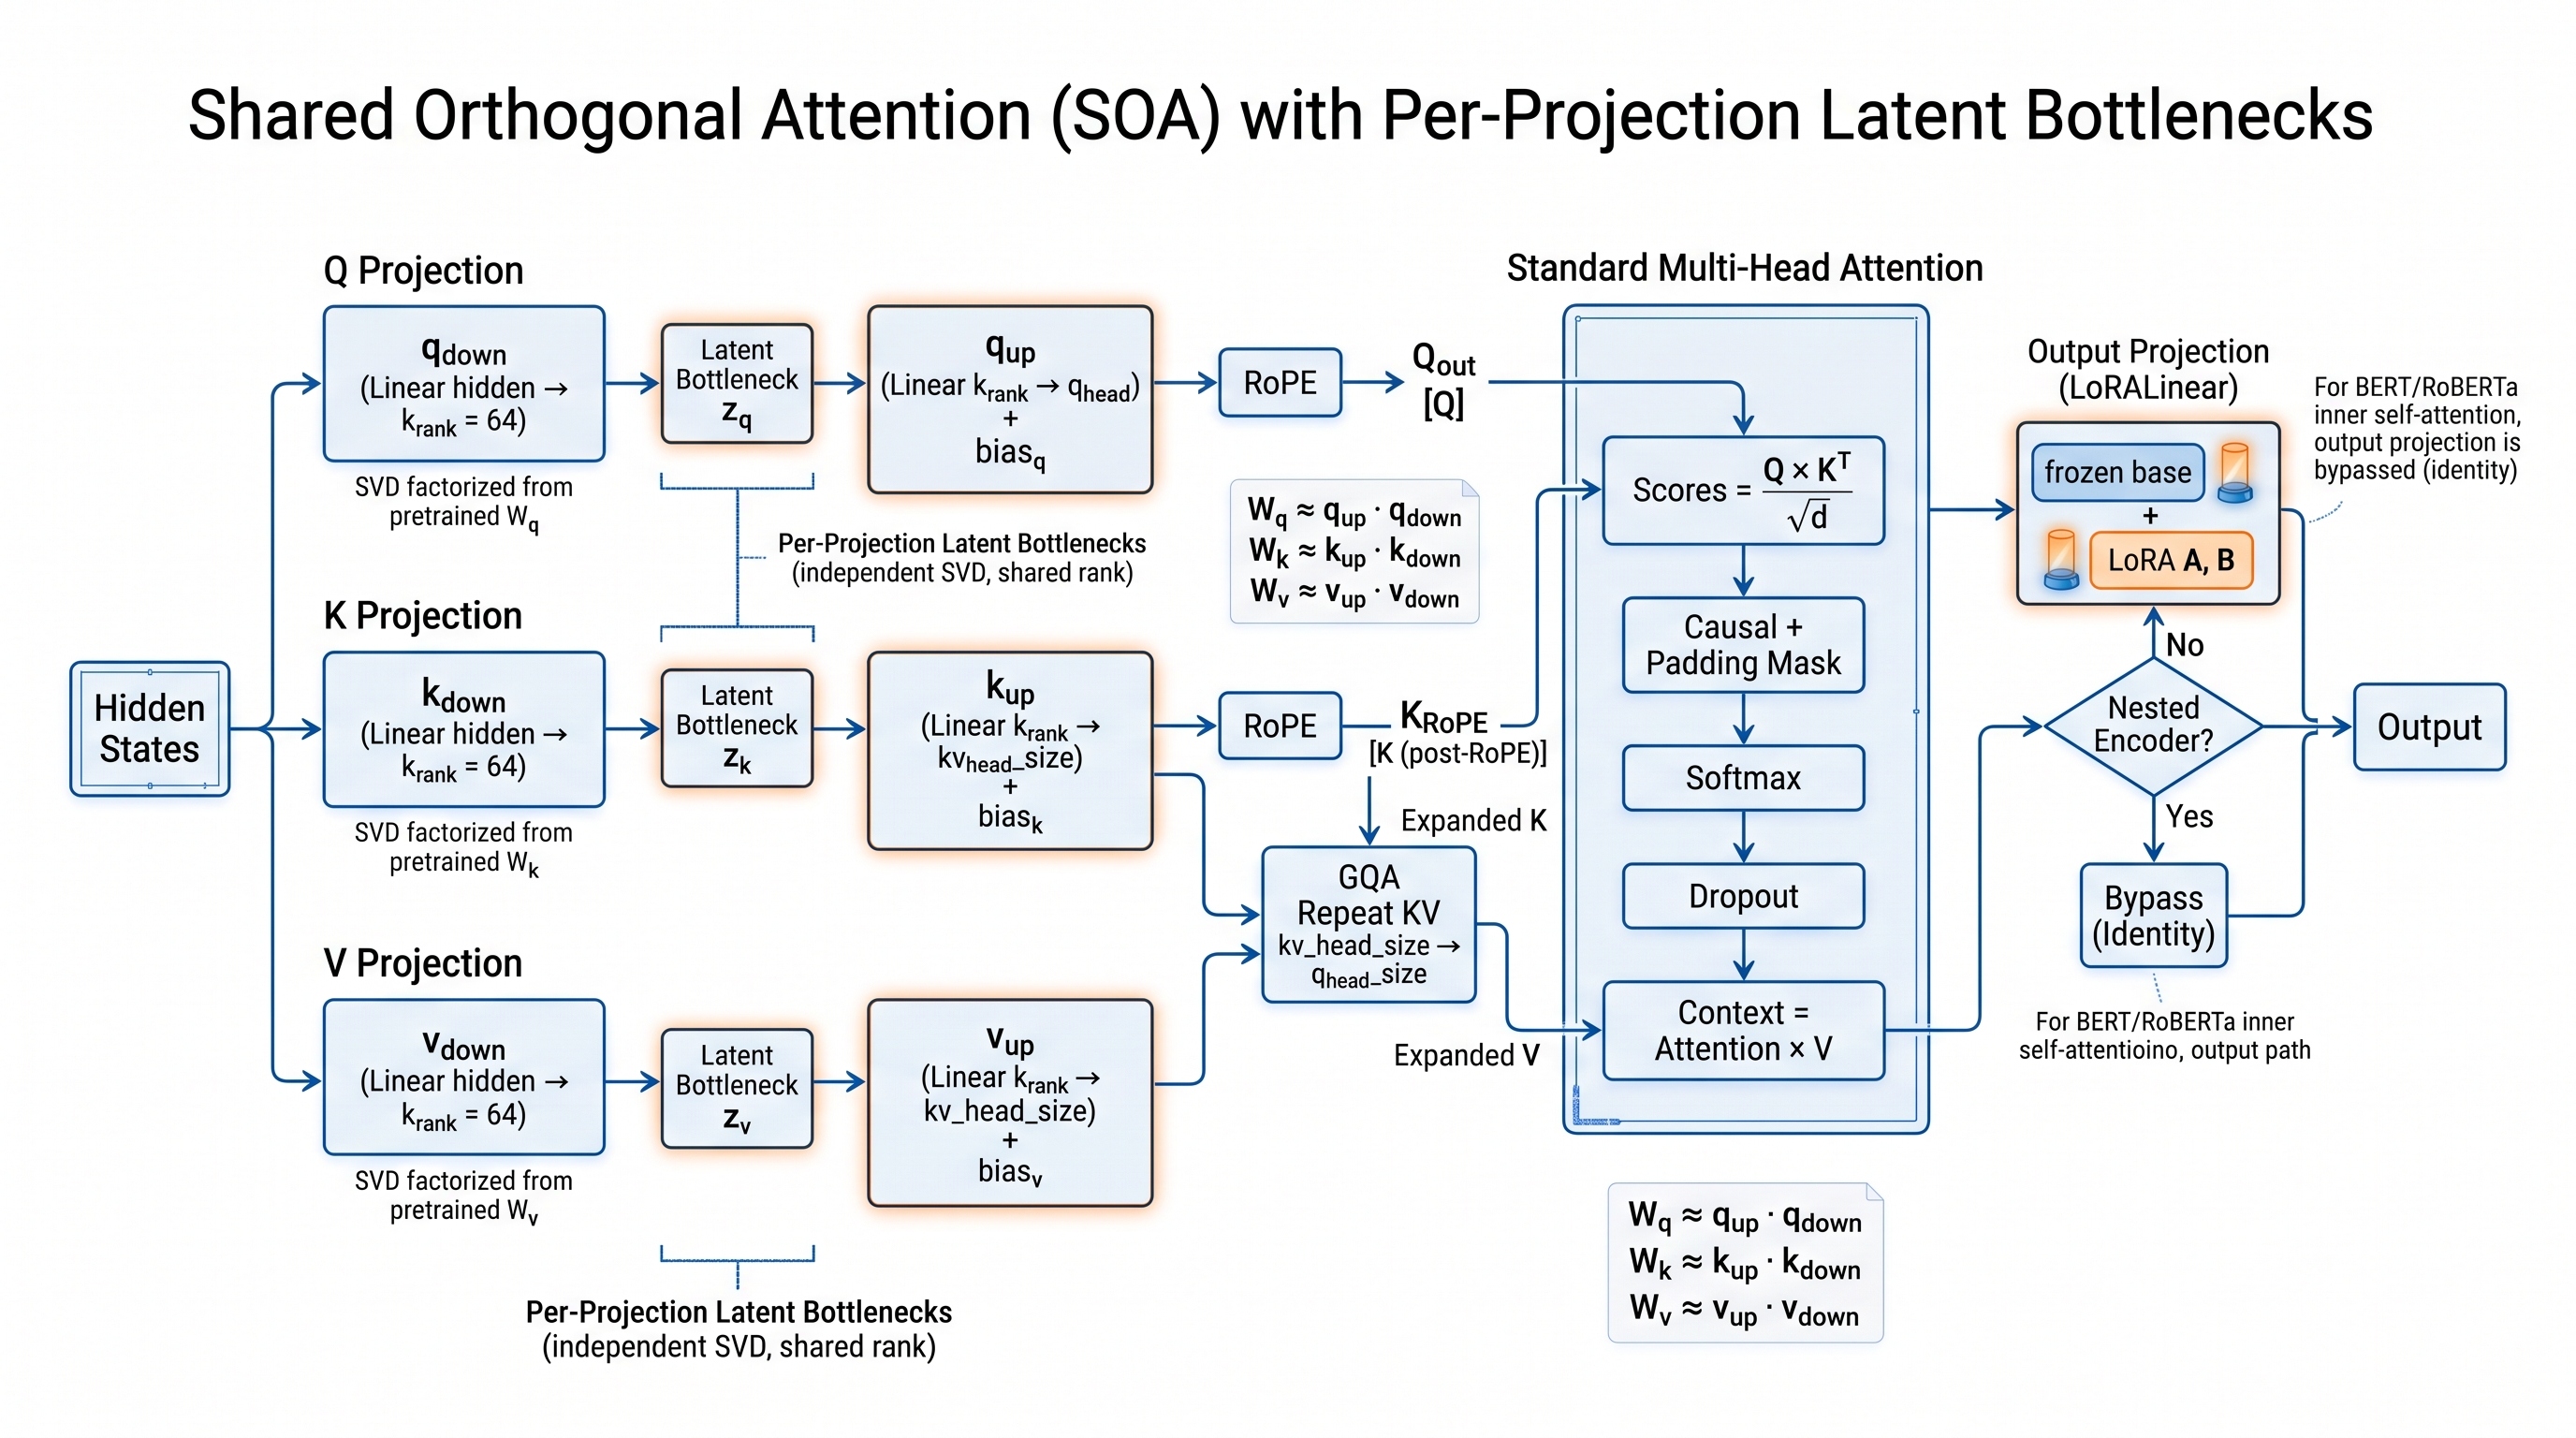
\includegraphics[width=0.92\textwidth]{img/arch_shared_orthogonal_attention.jpeg}
\caption{معماری توجه متعامد اشتراکی \lr{SOA (Shared Orthogonal Attention)} با تنگناهای نهان اختصاصی به ازای هر پروجکشن}
\label{fig:shared_orthogonal_attention_arch_soa_fused_module}
\end{figure}
